\documentclass[border=0pt]{standalone}
\usepackage{tikz}
\usetikzlibrary{decorations.pathreplacing,
  arrows,
  calc,
  decorations.pathmorphing,
  decorations.pathreplacing,
  decorations.markings,
  fadings,
  positioning,
  shapes
}
\tikzfading[name=fade img right,left color=transparent!100, right color=transparent!0]
\tikzfading[name=fade img left,right color=transparent!100, left color=transparent!0]
\tikzstyle{snakearrow} = [decorate, decoration={pre length=0.1cm,
  post length=0.1cm, snake, amplitude=.4mm,
  segment length=4mm},thick, ->]
\usepackage{graphicx}
\begin{document}
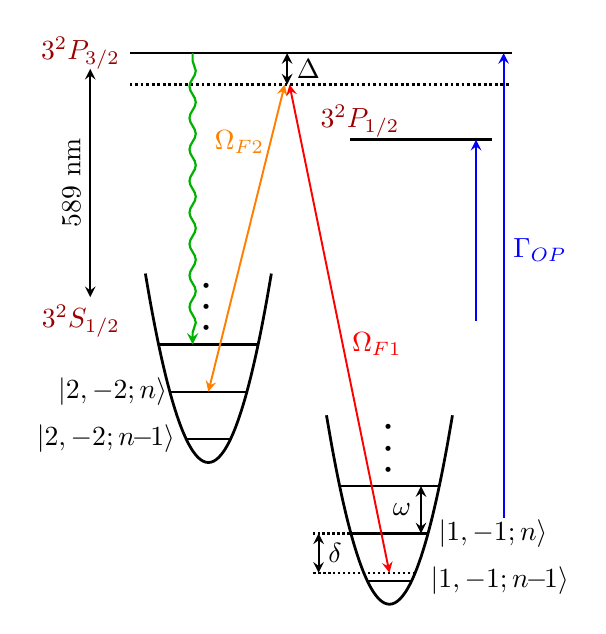
\begin{tikzpicture}
  % F2 trap
  \draw[line width=1]
  plot[domain={-0.8:0.8},smooth,variable=\x] ({\x}, {(\x)^2 * 3.75 - 1.2});
  \foreach \y in {0.3,0.9,1.5} {
    \draw[line width=0.8] ({-sqrt(\y / 3.75)}, \y - 1.2) -- ({sqrt(\y / 3.75)}, \y - 1.2);
  }
  \path (0, 1.5 - 1.2) node[right,rotate=90] {\LARGE $\cdots$};

  \path (-0.4, 0.9 - 1.2) node[left] {$|2,-2;n\rangle$};
  \path (-0.3, 0.3 - 1.2) node[left] {$|2,-2;n\!\!-\!\!1\rangle$};
  \path (-1, 0.6) node[left, red!60!black] {$3^2S_{1/2}$};

  % P3/2
  \draw[line width=1] (-1, 4.0) -- (3.85, 4.0);
  \draw[line width=1, densely dotted] (-1, 3.6) -- (3.85, 3.6);
  \draw[<->, line width=0.7, >=stealth] (1, 3.6) -- (1, 4.0);
  \path (1, 3.8) node[right] {$\Delta$};
  \path (-1, 4.0) node[left, red!60!black] {$3^2P_{3/2}$};

  % F2 Raman
  \draw[<->, line width=0.7, >=stealth, orange] (0, 0.9 - 1.2) -- (0.97, 3.6);
  \path (0.83, 2.6) node[orange,above left] {$\Omega_{F2}$};

  % D2 transition
  \draw[<->, line width=0.7, >=stealth] (-1.5, 0.9) -- (-1.5, 3.8);
  \path (-1.5, 2.35) node[above, rotate=90] {$589$ nm};

  % D2 decay
  \draw[snakearrow, >=stealth, green!70!black] (-0.2, 4.0) -- (-0.2, 0.3);

  % F1 trap
  \draw[line width=1]
  plot[domain={-0.8:0.8},smooth,variable=\x] ({\x + 2.3}, {(\x)^2 * 3.75 - 3});
  \foreach \y in {0.3,0.9,1.5} {
    \draw[line width=0.8] ({-sqrt(\y / 3.75) + 2.3}, \y - 3) -- ({sqrt(\y / 3.75) + 2.3}, \y - 3);
  }
  \path (2.3, 1.5 - 3) node[right,rotate=90] {\LARGE $\cdots$};
  \path (2.3 + 0.5, 0.9 - 3) node[right] {$|1,-1;n\rangle$};
  \path (2.3 + 0.4, 0.3 - 3) node[right] {$|1,-1;n\!\!-\!\!1\rangle$};

  % Raman det
  \draw[line width=0.8,densely dotted] (2.3, 0.9 - 3) -- (2.3 - 1, 0.9 - 3);
  \draw[line width=0.8,densely dotted] ({sqrt(0.4 / 3.75) + 2.3}, 0.4 - 3) -- (2.3 - 1, 0.4 - 3);
  \draw[<->, line width=0.7, >=stealth] (2.3 - 0.9, 0.9 - 3) -- (2.3 - 0.9, 0.4 - 3);
  \path (2.3 - 0.9, 0.65 - 3) node[right] {$\delta$};

  % F1 Raman
  \draw[<->, line width=0.7, >=stealth, red] (2.3, 0.4 - 3) -- (1.03, 3.6);
  \path (2.3 - 0.6, 0.3) node[red,right] {$\Omega_{F1}$};

  % Trap freq (F2)
  \draw[<->, line width=0.7, >=stealth] (2.3 + 0.4, 0.9 - 3) -- (2.3 + 0.4, 1.5 - 3);
  \path (2.3 + 0.4, 1.2 - 3) node[left] {$\omega$};

  % P1/2
  \path (1.3, 2.8) node[above right, red!60!black] {$3^2P_{1/2}$};
  \draw[line width=1] (1.8, 2.9) -- (3.6, 2.9);

  \draw[->, line width=0.7, >=stealth, blue] (3.4, 0.6) -- (3.4, 2.9);
  \draw[->, line width=0.7, >=stealth, blue] (3.75, -1.9) -- (3.75, 4.0);
  \path (3.75, 1.5) node[right, blue] {$\Gamma_{OP}$};
\end{tikzpicture}
\end{document}
